% -*- Mode:TeX -*-

%% IMPORTANT: The official thesis specifications are available at:
%%            http://libraries.mit.edu/archives/thesis-specs/
%%
%%            Please verify your thesis' formatting and copyright
%%            assignment before submission.  If you notice any
%%            discrepancies between these templates and the 
%%            MIT Libraries' specs, please let us know
%%            by e-mailing thesis@mit.edu

%% The documentclass options along with the pagestyle can be used to generate
%% a technical report, a draft copy, or a regular thesis.  You may need to
%% re-specify the pagestyle after you \include  cover.tex.  For more
%% information, see the first few lines of mitthesis.cls. 

%\documentclass[12pt,vi,twoside]{mitthesis}
%%
%%  If you want your thesis copyright to you instead of MIT, use the
%%  ``vi'' option, as above.
%%
%\documentclass[12pt,twoside,leftblank]{mitthesis}
%%
%% If you want blank pages before new chapters to be labelled ``This
%% Page Intentionally Left Blank'', use the ``leftblank'' option, as
%% above. 

\documentclass[12pt,twoside]{mitthesis}
\usepackage{lgrind}
\usepackage{graphicx}
\pagestyle{plain}

%% This bit allows you to either specify only the files which you wish to
%% process, or `all' to process all files which you \include.
%% Krishna Sethuraman (1990).
%
%\typein [\files]{Enter file names to process, (chap1,chap2 ...), or `all' to process all files:}
%\def\all{all}
%\ifx\files\all \typeout{Including all files.} \else \typeout{Including only \files.} \includeonly{\files} \fi

\begin{document}

% -*-latex-*-
% 
% For questions, comments, concerns or complaints:
% thesis@mit.edu
% 
%
% $Log: cover.tex,v $
% Revision 1.8  2008/05/13 15:02:15  jdreed
% Degree month is June, not May.  Added note about prevdegrees.
% Arthur Smith's title updated
%
% Revision 1.7  2001/02/08 18:53:16  boojum
% changed some \newpages to \cleardoublepages
%
% Revision 1.6  1999/10/21 14:49:31  boojum
% changed comment referring to documentstyle
%
% Revision 1.5  1999/10/21 14:39:04  boojum
% *** empty log message ***
%
% Revision 1.4  1997/04/18  17:54:10  othomas
% added page numbers on abstract and cover, and made 1 abstract
% page the default rather than 2.  (anne hunter tells me this
% is the new institute standard.)
%
% Revision 1.4  1997/04/18  17:54:10  othomas
% added page numbers on abstract and cover, and made 1 abstract
% page the default rather than 2.  (anne hunter tells me this
% is the new institute standard.)
%
% Revision 1.3  93/05/17  17:06:29  starflt
% Added acknowledgements section (suggested by tompalka)
% 
% Revision 1.2  92/04/22  13:13:13  epeisach
% Fixes for 1991 course 6 requirements
% Phrase "and to grant others the right to do so" has been added to 
% permission clause
% Second copy of abstract is not counted as separate pages so numbering works
% out
% 
% Revision 1.1  92/04/22  13:08:20  epeisach

% NOTE:
% These templates make an effort to conform to the MIT Thesis specifications,
% however the specifications can change.  We recommend that you verify the
% layout of your title page with your thesis advisor and/or the MIT 
% Libraries before printing your final copy.
\title{Incremental Random Forest Classifiers in Spark}

\author{Kathryn I. Siegel}
% If you wish to list your previous degrees on the cover page, use the 
% previous degrees command:
%       \prevdegrees{A.A., Harvard University (1985)}
% You can use the \\ command to list multiple previous degrees
%       \prevdegrees{B.S., University of California (1978) \\
%                    S.M., Massachusetts Institute of Technology (1981)}
\department{Department of Electrical Engineering and Computer Science}

% If the thesis is for two degrees simultaneously, list them both
% separated by \and like this:
% \degree{Doctor of Philosophy \and Master of Science}
\degree{Master of Science in Computer Science and Engineering}

% As of the 2007-08 academic year, valid degree months are September, 
% February, or June.  The default is June.
\degreemonth{June}
\degreeyear{2016}
\thesisdate{May 20, 2016}

%% By default, the thesis will be copyrighted to MIT.  If you need to copyright
%% the thesis to yourself, just specify the `vi' documentclass option.  If for
%% some reason you want to exactly specify the copyright notice text, you can
%% use the \copyrightnoticetext command.  
%\copyrightnoticetext{\copyright IBM, 1990.  Do not open till Xmas.}

% If there is more than one supervisor, use the \supervisor command
% once for each.
\supervisor{Samuel Madden}{Professor, EECS}

% This is the department committee chairman, not the thesis committee
% chairman.  You should replace this with your Department's Committee
% Chairman.
\chairman{Christopher Terman}{Chairman, Department Committee on Graduate Theses}

% Make the titlepage based on the above information.  If you need
% something special and can't use the standard form, you can specify
% the exact text of the titlepage yourself.  Put it in a titlepage
% environment and leave blank lines where you want vertical space.
% The spaces will be adjusted to fill the entire page.  The dotted
% lines for the signatures are made with the \signature command.
\maketitle

% The abstractpage environment sets up everything on the page except
% the text itself.  The title and other header material are put at the
% top of the page, and the supervisors are listed at the bottom.  A
% new page is begun both before and after.  Of course, an abstract may
% be more than one page itself.  If you need more control over the
% format of the page, you can use the abstract environment, which puts
% the word "Abstract" at the beginning and single spaces its text.

%% You can either \input (*not* \include) your abstract file, or you can put
%% the text of the abstract directly between the \begin{abstractpage} and
%% \end{abstractpage} commands.

% First copy: start a new page, and save the page number.
\cleardoublepage
% Uncomment the next line if you do NOT want a page number on your
% abstract and acknowledgments pages.
% \pagestyle{empty}
\setcounter{savepage}{\thepage}
\begin{abstractpage}
% $Log: abstract.tex,v $
% Revision 1.1  93/05/14  14:56:25  starflt
% Initial revision
% 
% Revision 1.1  90/05/04  10:41:01  lwvanels
% Initial revision
% 
%
%% The text of your abstract and nothing else (other than comments) goes here.
%% It will be single-spaced and the rest of the text that is supposed to go on
%% the abstract page will be generated by the abstractpage environment.  This
%% file should be \input (not \include 'd) from cover.tex.

This thesis presents a series of implementations of incremental random forests in Spark. My work draws from existing methods in online learning literature, but include several novel techniques. Through analysis of the performance of these implementations on varying workloads, I determine that tree regeneration is the best singular strategy for augmenting an existing random forest given an additional batch of training data. I also evaluate many hybrid strategies and show that regrowing a small proportion of trees is the best combined strategy with regards to time and performance. My results indicate that incremental growth strategies for online random forests are not useful for batched workflows. Overall, the system demonstrates significant performance gains when compared to the standard method of regrowing the random forest. 
\end{abstractpage}

% Additional copy: start a new page, and reset the page number.  This way,
% the second copy of the abstract is not counted as separate pages.
% Uncomment the next 6 lines if you need two copies of the abstract
% page.
% \setcounter{page}{\thesavepage}
% \begin{abstractpage}
% % $Log: abstract.tex,v $
% Revision 1.1  93/05/14  14:56:25  starflt
% Initial revision
% 
% Revision 1.1  90/05/04  10:41:01  lwvanels
% Initial revision
% 
%
%% The text of your abstract and nothing else (other than comments) goes here.
%% It will be single-spaced and the rest of the text that is supposed to go on
%% the abstract page will be generated by the abstractpage environment.  This
%% file should be \input (not \include 'd) from cover.tex.

This thesis presents a series of implementations of incremental random forests in Spark. My work draws from existing methods in online learning literature, but include several novel techniques. Through analysis of the performance of these implementations on varying workloads, I determine that tree regeneration is the best singular strategy for augmenting an existing random forest given an additional batch of training data. I also evaluate many hybrid strategies and show that regrowing a small proportion of trees is the best combined strategy with regards to time and performance. My results indicate that incremental growth strategies for online random forests are not useful for batched workflows. Overall, the system demonstrates significant performance gains when compared to the standard method of regrowing the random forest. 
% \end{abstractpage}

\cleardoublepage

\section*{Acknowledgments}

I would like to express gratitude towards my master's thesis advisor, Professor Sam Madden, for providing guidance on my project for the past year. I would also like to thank Manasi Vartak, whose advice and assistance has greatly contributed towards my research and results. 

%%%%%%%%%%%%%%%%%%%%%%%%%%%%%%%%%%%%%%%%%%%%%%%%%%%%%%%%%%%%%%%%%%%%%%
% -*-latex-*-

% Some departments (e.g. 5) require an additional signature page.  See
% signature.tex for more information and uncomment the following line if
% applicable.
% % -*- Mode:TeX -*-
%
% Some departments (e.g. Chemistry) require an additional cover page
% with signatures of the thesis committee.  Please check with your
% thesis advisor or other appropriate person to determine if such a 
% page is required for your thesis.  
%
% If you choose not to use the "titlepage" environment, a \newpage
% commands, and several \vspace{\fill} commands may be necessary to
% achieve the required spacing.  The \signature command is defined in
% the "mitthesis" class
%
% The following sample appears courtesy of Ben Kaduk <kaduk@mit.edu> and
% was used in his June 2012 doctoral thesis in Chemistry. 

\begin{titlepage}
\begin{large}
This doctoral thesis has been examined by a Committee of the Department
of Chemistry as follows:

\signature{Professor Jianshu Cao}{Chairman, Thesis Committee \\
   Professor of Chemistry}

\signature{Professor Troy Van Voorhis}{Thesis Supervisor \\
   Associate Professor of Chemistry}

\signature{Professor Robert W. Field}{Member, Thesis Committee \\
   Haslam and Dewey Professor of Chemistry}
\end{large}
\end{titlepage}


\pagestyle{plain}
  % -*- Mode:TeX -*-
%% This file simply contains the commands that actually generate the table of
%% contents and lists of figures and tables.  You can omit any or all of
%% these files by simply taking out the appropriate command.  For more
%% information on these files, see appendix C.3.3 of the LaTeX manual. 
\tableofcontents
\newpage
\listoffigures
\newpage
\listoftables


\chapter{Introduction}
Random forests have become one of the most popular machine learning classifiers
due to their robustness to noisy data, accuracy, and ability to handle "big
data" workloads. However, the downside to using random forests is that, given
additional training data, the random forest must be regrown from scratch. This
work proposes several techniques to update a random forest incrementally
without fully regrowing the classifier, as well as insight into the performance
and robustness of these techniques on different workloads. Specifically, I
explore incremental methods that are responsive to shifts in overall data
distribution. I develop a custom incremental random forest classifier and
provide a Scala API through which users can call incremental random forest
methods.

Chapter two describes the existing literature in online and incremental random
forests.

Chapter three describes the strategies I implemented for incrementally training
random forests.

Chapter four contains performance and robustness metrics for each of the random
forest implementations.

Chapter five describes a methodology for choosing a strategy for incremental
random forests, as well as the overlying system that intelligently chooses
between strategies at runtime.

Chapter six describes how my implementation fits into a larger system,
Sherlock, a data science tool for accelerating the process of model building. I
also address additional areas for research.

\section{Batched Workflows}

A common pattern in data science workflows involves training the same model on
increasing amounts of data. Such workloads are common in analytics, where
observations are continuously collected in log entries, as well as in Internet
of Things (IoT) networks, where extensive data collection takes place offline
and data is transmitted periodically. Existing machine learning tools retrain a
model on the entire dataset when new data is added. This entails reiterating
over every single data point in the dataset, even when the added batch has a
minimal effect on the resulting classifier. As such, implementing incremental
training in Spark random forests should drastically improve the performance of
these classifiers on batched workloads. This research seeks to implement and
expose a Scala API that will allow data scientists to add data to the random
forest using one of several incremental strategies. 

\section{Random Forest Classifiers}

This section introduces the mechanics of random forest classifiers. At a high
level, random forests are collections of decision trees used for
classification. Once grown, each decision tree classifies an unlabeled point by
casting a vote, and the random forest reports the label with the most votes.
\cite{Breiman}

My research involves the Spark Machine Learning (ML) implementation of random
forest classifiers. Apache Spark is a scalable system developed at Berkeley
that provides an engine for processing big data workloads. At its core is a
structure called the resilient distributed dataset (RDD), which can be
distributed over a cluster of machines and is fault-tolerant. A series of
powerful libraries run on Spark and take advantage of its powerful
cluster-computing capabilities. One such library is Spark MLlib, which contains
a wide array of machine learning tools. In this research, I model my
incremental random forest classifier on the Spark random forest classifier, for
the purposes of maintaining optimizations within the codebase that take
advantage of Spark's strengths. Since each batch in a batched workload may
contain a large dataset, implementing an incremental classifier in Spark allows
us to take advantage of Spark's distributed computing capabilities for every
batch.

The Spark ML random forest classifier favors batched and aggregated computation
over single-datapoint processing. Each dataset is first preprocessed into RDDs
with aggregated information about each point and its features. The Spark random
forest classifier then randomly samples the data (with replacement) according
to a Poisson distribution, and assigns a random sample to each decision tree in
the forest. Each decision tree is grown from the root using its sampled
dataset; the splitting criterion for each node in a decision tree is determined
with an element of randomness. Specifically, at each node, the set of features
is subsampled randomly. For each of the resulting set of features, the
classifier examines all possible values for that feature on which the data can
be split. Among all of these candidate splits, the classifier chooses the split
that maximizes the decrease in Gini impurity-{}-the probability that a point
randomly selected from the node would be misclassified. The algorithm
terminates when the maximum tree height is reached or no training points are
misclassified within each individual decision tree.

The existing Spark ML random forest classifier performs well given a large
dataset. However, like all implementations of random forests, a change in the
training dataset would mean retraining the random forest from scratch.
Retraining from scratch would lead to a lot of repetitive computation; the
aggregate composition of the dataset might not change significantly with the
new batch, especially if each batch has far fewer data points than the overall
dataset. This thesis presents work that allows random forest classifiers to be
updated with each new batch of training data more efficiently, therefore saving
time for data scientists and other users of Spark MLlib.

\chapter{Previous Work} Since Leo Breiman introduced random forests to the data
science community in 2001 \cite{Breiman}, researchers have tested various
refinements of the algorithm. One area of focus has been augmenting the
algorithm for online learning. This chapter describes the existing literature
on incremental and online random forests.

\section{Ensemble models} A random forest is a type of ensemble model, which
average the predictions of many different ``reasonably good'' models to produce
a prediction that better estimates the true hypothesis. Ensemble models are
highly successful as machine learning tools, because they avoid the
chance-dependent pitfalls of many singular models. For example, gradient
descent methods can get stuck in local minima, but combining many models
increases the chance that one will find the global minimum. Alternatively, even
if none of the models in the ensemble  produce the true hypothesis, averaging
every prediction can lead to a a prediction that more closely matches the
underlying truth. \cite{Dietterich}

There are several established methods for aggregating model predictions in
ensembles. The Bayesian voting algorithm iterates through all hypotheses
produced by models in the ensemble, and then combines the results based on how
likely the hypothesis is given the sample. Another method is to manipulate the
training data via bagging, known as bootstrap aggregation, and boosting, known
as weighted training. Bagging involves randomly sampling points with
replacement from a common dataset; the default Spark implementation of random
forests uses bagging over boosting. Other ensemble methods exist but are not
utilized in Spark ML.


\section{Online random forests} Standard random forests are offline
classifiers; trees are built on static datasets. Offline classifiers are poorly
suited for datasets for which additional data points become available
incrementally. A prevalent example is logging; logs are published as actions
take place within a system, and a classifier for these logs must take into
account the new information to avoid becoming inaccurate. Similar problems
requiring an online classifier are found throughout industry. For example,
Yahoo uses an online classifier to characterize relevant articles to show each
user on its homepage. In many of these use cases, retraining the classifier
from scratch would take an excessive amount of time, given the enormous amount
of existing training data. Since new batches of data are often far smaller than
the size of the aggregate training data, the new data only shifts a
classifier's behavior slightly. Retraining an entire classifier from scratch to
capture slight shifts seems wasteful; online classifiers provide a far more
efficient approach.

In this thesis, I study incremental random forest classifiers--forests that
update themselves with new batches of data. Incremental forests are a subset
online random forests; they are updated with new batches of data, rather than
with one new point at a time. Batched updates can take advantage of Spark's
strength, which is distributed, batched computation. Simply implementing an
online random forest classifier in Spark would be computationally wasteful, as
it would require a new Spark job for every additional point. Focusing on
batched updates plays to Spark's strengths and addresses a sparser area of the
machine learning literature. Existing online methods are easily extended into
batched methods, and batched computation provides an opportunity for
optimizations.

\subsection{Saffari online random forests} The most well-known implementation
of an online random forest is the Saffari implementation. \cite{Saffari} In
offline mode, a Saffari random forest behaves like a typical random forest:
each tree is created by sampling the original training set, the split at each
node is chosen as the best among a random set of feature candidates, and
predictions are made by summing conditional probabilities among all of the
trees.

In online mode, trees receive a serial string of points and are grown in an
extremely randomized fashion; at every node, tests and thresholds are chosen
randomly. Specifically, when a node is created, it establishes a set of N
random tests and maintains statistics on the left and right partitions created
by each test. When a new point is added to the tree, the point's features place
it in a leaf node. The algorithm then recalculates the gain $\mathrm{G_n}$ with
respect to each test in that node $n$ according to the following equation:
\begin{equation} \mathrm{G_n}=\ell_n - \frac{|samples_l|}{|samples_n|}*\ell_l -
\frac{|samples_r|}{|samples_n|}*\ell_r, \end{equation} where $\ell$ indicates
loss, $l$ represents the left partition of a split, and $r$ represents the
right partition of a split. The Saffari algorithm splits a leaf based on two
hyperparameters: $\alpha$, the minimum number of samples a node must see, and
$\beta$, the minimum gain a split must achieve. When both conditions are
satisfied, the node splits.

The Saffari algorithm also specifies that trees can be discarded randomly,
where the probability that a tree is discarded increases with its out-of-bag
error. This trait allows the random forest to adapt to changes in the data
distribution.

Saffari claims this algorithm is better than alternatives such as the Hoeffding
tree algorithm (addressed later in this chapter), because it fits better to the
inherent nature of decision trees. Empirically, Saffari random forests perform
better than boosted forests. In my research, I test the efficacy of using the
extremely randomized trees of the Saffari algorithm. I also experiment with the
aforementioned split hyperparameters, tweaking my algorithm to select more
optimal gain and points thresholds. Since the Spark random forest
implementation closely matches the Saffari offline random forest
implementation, many of my initial modifications to the Spark code to provide
online learning capability are in line with the Saffari online-mode algorithm.

\subsection{Denil online random forests} In "Consistency of Online Random
Forests," Misha Denil et al. proposes and evaluates improvements to the Saffari
online random forest algorithm. Denil online forests partition the sequence of
data points into ``structure'' points and ``estimation'' points. \cite{Denil}
Structure points influence the structure of the tree but do not affect the
predictions made in tree leaves. Estimation points do not influence the
structure of the tree, but are used to re-estimate probabilities. The Denil
algorithm uses the same split selection procedure as the Saffari algorithm. The
paper shows that this refined implementation achieves a higher accuracy on
complex datasets compared to a comparable implementation of the Saffari
algorithm.

Much of the existing literature around online random forests acknowledges one
primary setback: due to decision trees’ recursive structure, lower data cannot
be used to correct earlier decisions. Both the Saffari and the Denil
implementations have this flaw. The new few subsections address algorithms that
involve regrowing part or all of select decision trees within a random forest.
My research draws on both classes of techniques-{}-incremental growth and
regeneration.

\subsection{Mondrian forests}

Another type of online random forest is a Mondrian forest \cite{NIPS2014_5234},
which are comprised of augmented extremely randomized decision trees. The
algorithm for building each Mondrian decision tree is as follows.  We start at
the root and allocate a budget, $\lambda$, for this node. Then, we recursively
process each node by randomly choosing split locations on the ranges of feature
values. For each point $j$, dimension $d$, and dimension-wise maximum and
minimum $u_{jd}$ and $l_{jd}$, let $E = \sum_d(u_{jd}-l_{jd})$. Then, these
cuts each cost $\lambda' = \lambda - E$. If we can ``afford'' the cut, we split
the node and assign budget $\lambda'$ to each subinterval. The tree stops
growing when no more cuts can be afforded at any leaf node. Throughout the
growing process, we denote a split hierarchy using a time variable. A node's
time variable $\tau$ is set when a split is made within that node; the value of
this variable is equivalent to $E + \tau_{parent}$. 

To adapt Mondrian trees for online learning, we use the time parameter to
determine where a new cut should be inserted. Starting at the root, we recurse
down the tree until the cost coefficient $E_{new}$ for this new node is less
than the cost coefficient $E_{old}$ for some node. We then insert the new node
as the parent of this old node and adjust all children nodes accordingly.

Mondrian forests achieve an accuracy very close to offline Breiman random
forests and extremely randomized forests trained on the same fraction of the
data. The Mondrian algorithm significantly outperforms the Saffari algorithm
when trained in online mode on the same fraction of data. Furthermore, Mondrian
forests were shown to adapt to new data an order of magnitude faster than
simply regrowing a forest from scratch.

The drawbacks of Mondrian forests include its relative intolerance of
irrelevant data. Because splits are random, irrelevant and relevant features
are equally likely to be chosen; noisy features can then harm the overall
accuracy of each tree. Additionally, a Mondrian forest in online mode might
choose to insert a node close to a root, thus initiating recalculation of a
large section of the tree.

While Mondrian forests outperform Saffari online random forests, regrowing a
tree section requires passing through all of the data points yet seen. As
datasets grow larger, the overhead incurred by additional passes through the
data will outweight the efficiency gains of the algorithm. Mondrian forests
have only been shown as more efficient than Saffari online random forests on
datasets of a few thousand data points. As such, the optimal strategy should
regrow parts of a random forest but should not require multiple passes over the
data.

\section{Concept drift} Concept drift describes changes in data distribution in
an online learning setting that cause the mathematical relationships between
the input variables and output predictions to change. These shifts cause ML
classifiers trained on earlier data points to become inaccurate. The online
random forest algorithms discussed earlier in this chapter adapt poorly to
concept drift, as they accommodate new data by splitting leaves or regrowing
small sections of trees in the forest. Concept drift can cause splits in nodes
higher in the trees to become inaccurate, and a poor decision higher in the
tree more significantly impacts performance than a mistake closer to the
bottom. Online random forests adapt more poorly than other online classifiers
to concept drift, as splits made in nodes are essentially permanent. In
contrast, classifiers that use, for example, linear or logistic regression
could just shift internal weights until the concept drift is accounted for.

Therefore, accounting for concept drift in online random forests requires
regrowing trees--the decisions from these trees must counteract bad decisions
from other trees resulting from wrong splits. Purely incremental strategies, or
those that just split leaves, should not be the only methods by which online
random forests adapt to change.

\section{Combined strategies} Several papers in the literature use Hoeffding
trees to grow online random forests. Hoeffding trees for online learning were
first proposed in a paper by Domingos and Hulten; when growing, these trees
maintain several candidate splits in each leaf, with the quality of each split
estimated in an online manner. \cite{Domingos} In contrast with the minimum
gain parameter controlling splits in Denil and Saffari random forests,
Hoeffding trees use a measure of the Hoeffding bound to ensure that a split is
optimal. Hoeffding trees split leaves when the Hoeffding bound indicates that
the current best split is the optimal split, within reasonable certainty. 

A paper by Bifet et al. describes an implementation of the Hoeffding tree
algorithm that adapts to concept drift. \cite{Bifet} The algorithm grows
Hoeffding trees of different sizes; the authors reason that smaller trees can
adapt more quickly to concept drift, whereas larger trees are less sensitive to
noisy deviations. The trees are occasionally either partly or fully regrown,
depending on a metric called ADWIN that estimates drift. The Bifet paper's
results show that the method is effective on small generated datasets with
concept drift.

Abdusalam et al. developed an algorithm that grows random forests incrementally
by using Hoeffding trees and selecting entire trees for replacement. Unlike the
algorithm from the paper by Bifet et al., the system chunks a data stream, then
processes data chunks serially. The algorithm detects concept drift using a
two-window technique; if a tree's classification error between the two windows
differs by an amount less than a threshold, it is not grown further. Otherwise,
grow the tree incrementally. With every given batch, 25\% of the trees are
automatically regrown, with additional trees regrown if the system detects
concept drift.

I take into account these algorithms when developing my system in Spark.
Namely, my implementation heavily involves a balance between incremental growth
and tree replacement, much like the algorithms in the Bifet and Abdusalam
papers. I refer back to these previously-developed algorithms in my discussion
of the Spark incremental random forests system developed in this thesis.

\chapter{Methods} This chapter describes the two main strategies I implemented
for incrementally training random forests. I go into depth about the details of
each implementation, hybrid strategies, and the API I exposed for use in Spark
ML pipelines. My experiments seek to shed insight into which algorithms work
best on different workloads.

\section{Tree regeneration strategy}

The first implemented strategy involves regrowing trees within the random
forest. For every new incremental batch, the exposed Spark API allows an
existing model to be updated with the new data. A set proportion of trees are
randomly selected for replacement. The system then grows a random forest with
the number of trees selected, and creates a new hybrid model with the
maintained trees from the old model and the newly grown trees from the new
model. To allow for the creation of hybrid models, I introduce an incremental
random forest classification model. This model tracks metadata from
previously-seen data and information about each tree in the forest. 

\section{Incremental growth strategy}

The second implemented strategy involves incrementally growing existing trees
in the forest, and is based off of the Saffari and Denil algorithms. A user can
update an existing incremental random forest classification model with a new
batch of data via the exposed Spark API. Because this model tracks metadata
from previous batches of data, the system can determine the candidate splits
that were considered during previous growth phases of the tree. The new data is
divided into bins specified by the previously-calculated splits and used to
split leaves of the tree.

I augmented the RandomForest class in Spark ML to store metadata about past
runs in leaves. Specifically, the random forest metadata maintains a list of
data splits by feature; these splits determine the ``bins'' to which each new
point belongs. After the new batch of data is processed into bins, I merge this
information with the information stored in each leaf. To provide leaves with
ability to store metadata and merge in new batches of data, I implemented a
custom incremental leaf node class that replaces the customary Spark-provided
leaf node class. This class maintains the capabilities of the original Spark
leaf node, but allows for changes to be made to each tree in the random forest.

Once the new metadata is aggregated at each leaf, the system splits leaves that
newly pass both requisite thresholds: the minimum number of points a leaf must
account for and the minimum information gain from the split. After each tree is
incrementally grown, the system returns a new incremental random forest model
with updated metadata to the user.

\section{Optimizations}

\subsection{Bounding incremental growth}

Since datasets can have many features, unbounded tree growth can result in
extremely deep trees after just a few batches. The largest tree height
supported by Spark ML is 30, after which trees can no longer be grown
incrementally. Additionally, splitting leaves in tall trees imposes a large
performance overhead, as the algorithm must examine a large number of candidate
leaves. As a result, the system restricts the maximum initial tree height to a
set value $h$, relaxing this restriction by one for each incrementally grown
tree that receives a new batch of data. In all hybrid strategies, a tree is
replaced when it reaches a certain threshold depth. When a tree is regrown, its
maximum height is reset to the original value $h$. This technique prevents the
incremental random forest from overfitting to earlier batches and allows the
forest to better adapt to concept drift, as it ensures that later batches can
significantly impact tree predictions.

\subsection{Batched processing}

The incremental random forest implementations in the Saffari and Denil papers
describe accumulating points in leaves until the leaf is split. In the purely
online setting, accumulating points one at a time is the only option. Since
batched workloads allow for many points to be processed at one time, we can
preprocess the batch into metadata structures that are passed to the relevant
leaves and merged with the existing leaf metadata. This optimization prevents
the system from having to run back over all previous batches to decide on a
split.

\subsection{Tree reweighting}

In the batched incremental learning setting, the classifier receives an
unlabeled batch of points, predicts the label for each point, and then views
the labels to assess its accuracy. Each tree in the random forest has a
different accuracy on a particular new batch of data. To increase the overall
accuracy of the forest, after the system assesses the accuracy on each new
batch, it weights the trees with lower accuracy to have less voting power on
the next batch. Because this increases the chances of overfitting, the system
restricts the extent to which tree weights can shift.

To account for concept drift, I weight trees by age. With every new batch,
trees that are not regrown are weighted to have less voting power. As a result,
the classifier captures information from previous batches, but uses information
from the most recent batch more heavily in the classification of the next
batch.

\subsection{Leaf subsampling}

As tree height increases, the amount of computation required to grow the tree
one level increases significantly. However, adapting an existing tree to a new
batch of data does not necessarily require splitting every leaf in the the tree
on the new data. Instead, the system can select a random sample of the leaves
in the tree, and only consider these leaves for incremental growth. While this
optimization decreases the performance of shallow random forests, for deep
forests, it helps improve the training time without significantly impacting the
performance.

\section{Hybrid approach}

The tree regeneration and incremental growth strategies are compatible; both
can be used simultaneously within an incremental random forest. This thesis
explores various hybrid approaches and provides insight into which approaches
work best on datasets with and without concept drift. For each hybrid approach,
I vary the proportion of trees that are grown with each strategy. The system
selects trees without replacement to be replaced or grown incrementally; the
remaining trees are unchanged. I also implement several optimizations for this
approach that are applied to all trees after every batch.

% TODO

\section{Experiments}

In my research, I experiment with several different parameters that affect the
error rate of my incremental random forest classifier. I hypothesize that
certain parameters used to build each incremental random forest will affect the
optimal incremental strategy for that forest on my test datasets. I vary the
following parameters in my experiments and report the effect on the optimal
hybrid incremental algorithm.

\begin{enumerate}

    \item \textbf{Tree depth.} I vary the initial maximum height of each tree
      in the random forest. In my experiments, I use two initial heights:
      shallow and deep, which represent heights of 5 and 10, respectively. I
      chose 10 to be the sample height for deep trees, as it is the most
      commonly used height in the literature to obtain a high accuracy without
      overfitting. A shallow tree height of 5 still provides some accuracy, but
      allows the tree to adapt more significantly to concept drift in
      incremental batches. 

    \item \textbf{Tree count.} I vary the number of trees in the forest. In my
      experiments, I test two tree quantities: narrow and wide, which represent
      tree counts of 10 and 100, respectively. These two tree quantities are
      most common in the literature; 10 trees are used when training time is a
      large concern, whereas forests with 100 trees are typically more
      accurate.

    \item \textbf{Concept drift.} I test the performance of the incremental
      random forest classifier on two datasets: one with concept drift and one
      without concept drift. The dataset with concept drift is sampled from the
      United States Department of Transportation Airline On-Time Statistics and
      Delay Causes dataset; the classifier predicts whether a flight is
      delayed, and flight delays naturally shift over the course of a year.
      \cite{Plane} The dataset without concept drift is from the Homesite Quote
      Conversion Kaggle competition; the classifier predicts whether a quote
      will convert into a purchase. \cite{Homesite}

\end{enumerate}

\section{API}

My custom incremental random forest classifier class,
IncrementalRandomForestClassifier, exposes a Scala API for data scientists to
use. I introduce a new model class, the
IncrementalRandomForestClassificationModel class, which is an augmented
adaptation of the Spark ML RandomForestClassificationModel class that allows
for incremental optimizations. The table in figure \ref{tab:api} details the
methods available for use in Spark ML pipelines.

\begin{table}
  \centering
  \begin{tabular}{ | c | c | }
  \hline
  \textbf{Method} & \textbf{Description} \\
  \hline
  def train(df: DataFrame): & Trains a model for future \\
  IncrementalRFClassificationModel &  online learning by maintaining \\
  & tree and leaf metadata. \\ 
  \hline
  def update( & Updates an existing model \\
  old: IncrementalRFClassificationModel, & with a new batch of data \\
  df: DataFrame): & by regrowing some trees and \\
  IncrementalRFClassificationModel & incrementally growing others. \\
  \hline
  def addTrees( & Trains a model using a warm \\
  oldModel: IncrementalRFClassificationModel, & start by adding more \\
  df: DataFrame, addedTrees: Int): & trees to the existing forest. \\
  IncrementalRFClassificationModel & \\ 
  \hline
  def setRegrowProportion(prop: Int) & Set the proportion of trees \\
  & in the forest that should be \\
  & regrown with every new batch. \\
  \hline
  def setIncrementalProportion(prop: Int) & Set the proportion of trees \\
  & in the forest that should be \\
  & regrown with every new batch. \\
  \hline
  def setInitialMaxDepth(depth: Int) & Set the initial depth of \\
  & newly-grown trees. \\
  \hline
  \end{tabular}
  \caption{Scala API for the incremental random forest (RF) classifier developed in this thesis.}
  \label{tab:api}
\end{table}

\chapter{Results} In this chapter, I analyze the benchmark results and discuss
their implications for data scientists using incremental random forest
classifiers. In each trial, each incremental random forest classifier received
batches sequentially, retraining itself after every new batch. For each tested
workload, I first contrast the performances of the incremental growth and tree
replacement strategies, and then I analyze a range of hybrid strategies and
explore the ideal hybrid strategy based on concept drift.

% TODO ERF


\section{Workload A: Large batches, no concept drift}

The Homesite Quote Conversion dataset is a Kaggle dataset that provides over
fifty numerical and categorical metrics on each of 200,000 customers. The
classification goal is to determine whether a potential customer will purchase
home insurance given the provided metrics about their quoted price, previous
activity, coverage information, and more. \cite{Homesite}

To study how incremental random forests would perform on workloads with large
batch sizes and no concept drift, I randomly divided the Homesite dataset into
ten batches of 20,000 data points each, and ran tests using both deep and
shallow random forests. By contrasting the error rates over time, I provide insight
into how these forests adapt over time.

\begin{figure}
  \centering
  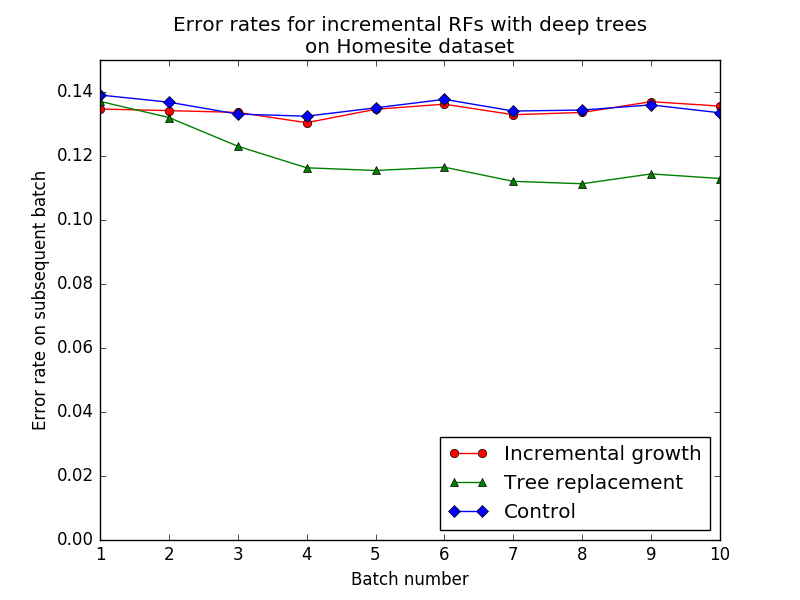
\includegraphics[width=4.0in]{g1}\\
  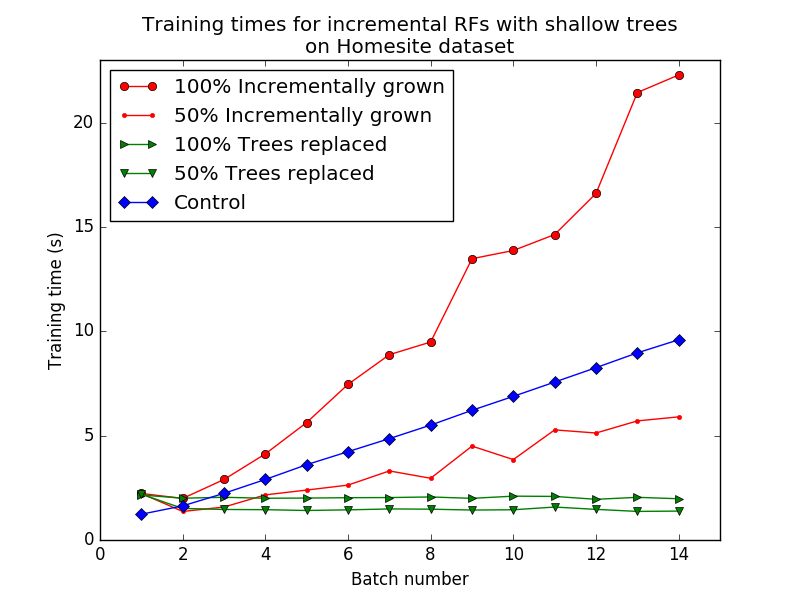
\includegraphics[width=4.0in]{g1_1}
  \caption{These graphs show the error rates and training times for the
  incremental growth strategy, the tree replacement strategy, and the control
  setting on the batched Homesite Quote Conversion dataset. In this benchmark,
  the random forest classifiers grow deep trees.}
  \label{fig:homesite}
\end{figure}

\begin{figure}
  \centering
  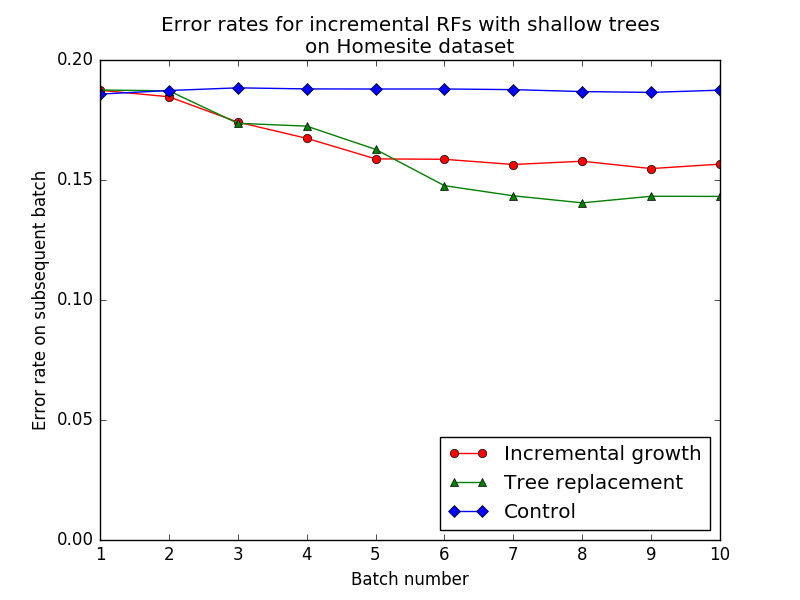
\includegraphics[width=4.0in]{g2}\\
  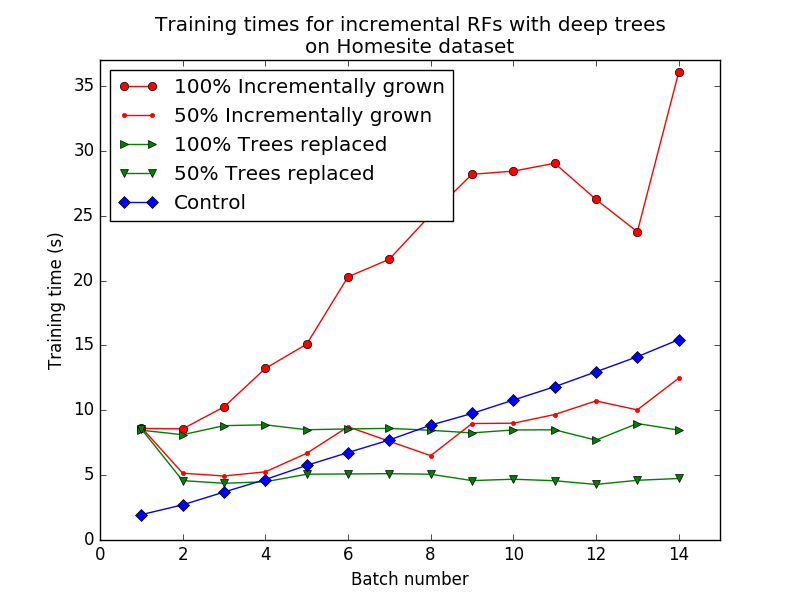
\includegraphics[width=4.0in]{g2_1}
  \caption{As with the graphs on the previous page, these graphs show the error
  rates and training times for the two experimental strategies, as well as the
  control. This benchmark, in contrast, measures random forest classifiers grown
  with shallow trees.}
  \label{fig:homesite2}
\end{figure}

As seen in Figures \ref{fig:homesite} and \ref{fig:homesite2}, in forests with
deep trees, the incremental growth strategy performed just as well as the
control, while the tree replacement strategy achieved an error rate over $2\%$
lower.  Because each batch contained 20,000 data points, the random forest
classifier was able to fit the data distribution accurately by just training on
the first batch of data. Since the dataset exhibited no concept drift, once the
data distribution was learned to a sufficient degree of accuracy, incrementally
growing each tree on new batches did not change the classification behavior of
the forest. As a result, the incremental growth strategy did not improve the
performance of the random forest. Similarly, incorporating each additional
batch into the tree by regrowing from scratch did not improve the accuracy of
the random forest.  However, the tree replacement strategy was able to better
fit to the data over time by replacing the trees with a lower overall
classification accuracy; since the batch size was large, if a tree had poor
classification performance on one batch, it likely would have poor performance
on future batches.

In contrast, in forests with shallow trees, the incremental growth strategy
performed far superior to the control, and almost as well as the tree
replacement strategy. Shallow trees more easily adapt to new data; in
traversing a decision tree from the root to a leaf, the information gain in
each leaf necessarily decreases with every level. Initially growing shallow
trees allows for future batches to more significantly impact the decisions made
by the forest.

As expected, retraining the entire tree from scratch on all data caused the
training time for the control setting to be much higher on later batches than
the training time for the experimental settings. The training times for the
incremental growth strategy were slightly smaller than the times for the tree
replacement strategy, regardless of tree depth.

Overall, for workloads such as the Homesite Quote Conversion batched dataset, a
large batch size and stationary distribution of data points indicates that a
pure replacement strategy is optimal to minimize error rate. 

TODO hybrid strategies

\begin{figure}
  \centering
  TODO
  \caption{These two plots show the average error rates of various hybrid tree
  replacement and incremental growth strategies on the Homesite batched
dataset. The axes indicate the percentage of trees that are modified according
to each strategy.}
  \label{fig:homesitehybrid}
\end{figure}

\section{Workload B: Small batches, no concept drift}

The Otto Group Product Classification dataset contains 200,000 data points
representing products sold by the Otto Group. Each data point is characterized
by nearly 100 numerical features representing qualities of each product; the
classification task is to distinguish one particular product category, ``Class
2,'' from the others. By randomly downsampling the dataset, I segmented the
data into batched workloads of approximately 100 points per batch, much smaller
than the 20,000-point batches of the Homesite dataset. \cite{Otto}

My initial analysis, as with the Homesite dataset, involved contrasting the
performance of the two incremental random forest strategies on the data. I
trained random forest classifiers using each of the two strategies on fifty
100-point batches of the Otto dataset to demonstrate any trends over time.

\begin{figure}
  \centering
  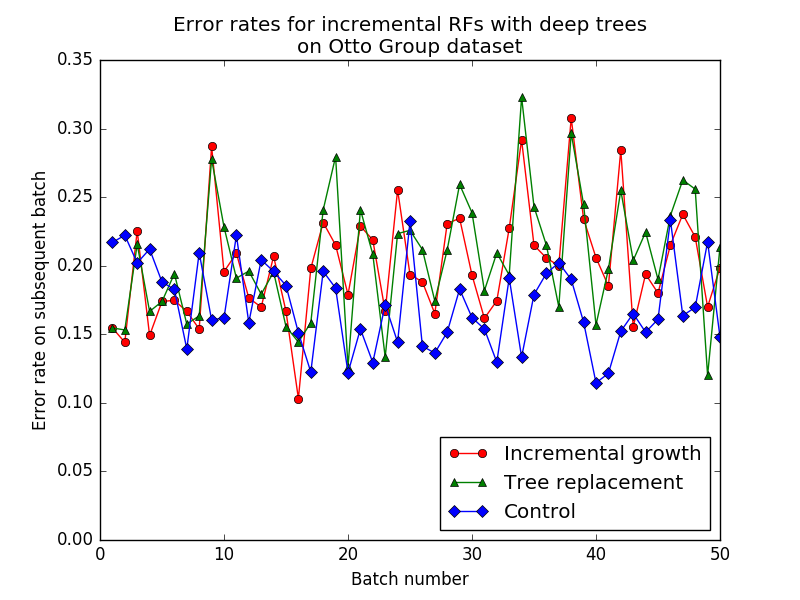
\includegraphics[width=4.0in]{otto3}\\
  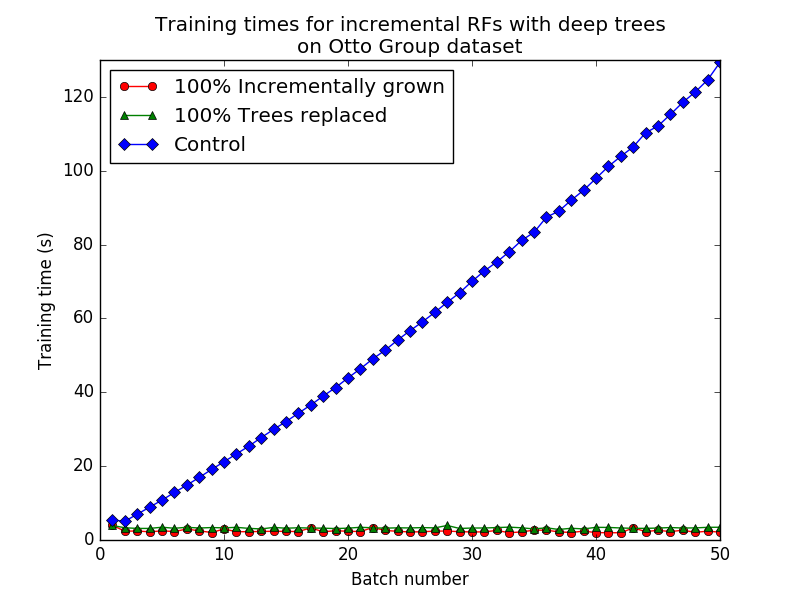
\includegraphics[width=4.0in]{otto4}
  \caption{These graphs show the error rates and training times for the
incremental growth strategy, the tree replacement strategy, and the control
setting on the batched Otto Group Product Classification dataset. These metrics
were taken on online random forest classifiers growing deep trees.}
  \label{fig:otto1}
\end{figure}

\begin{figure}
  \centering
  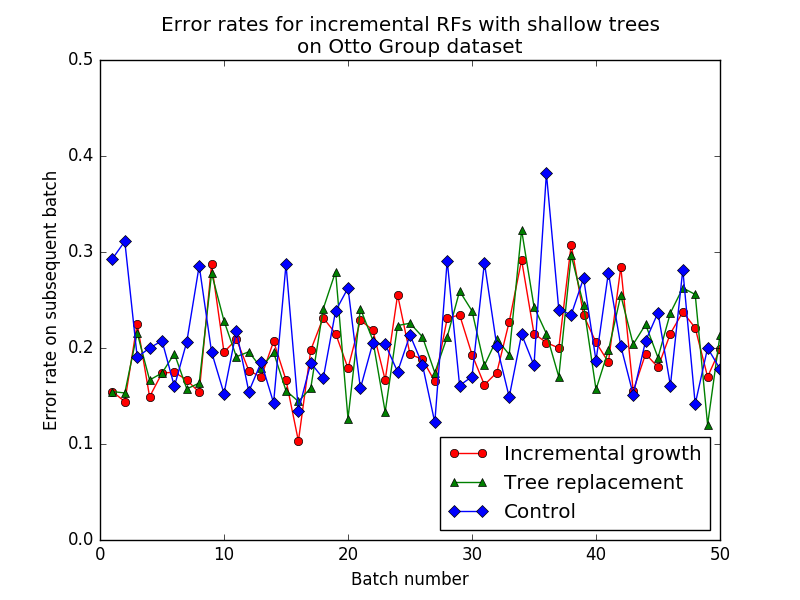
\includegraphics[width=4.0in]{otto1}\\
  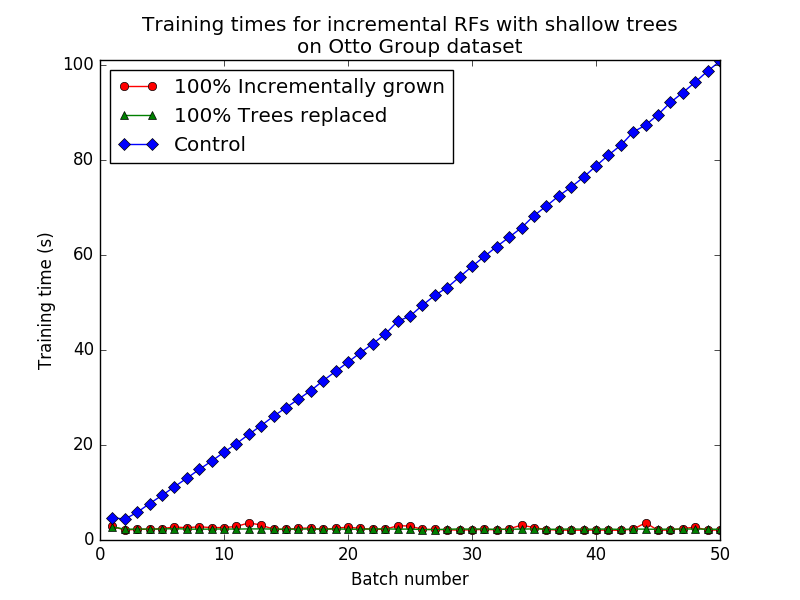
\includegraphics[width=4.0in]{otto2}
  \caption{As in the previous figure, these graphs show the error rates and
    training times for the two experimental strategies and the control on the
    Otto Group dataset. These benchmarks were measured on online random forest
  classifiers growing shallow trees.}
  \label{fig:otto2}
\end{figure}

As seen in Figures \ref{fig:otto1} and \ref{fig:otto2}, unlike with the Homesite
workload, there is no pure strategy that demonstrates the lowest error rate
across all batches. This observation is consistent both in random forest
classifiers with deep trees and in those with shallow trees. As expected, the
control again demonstrates the largest training time after each batch, as it
must be retrained from scratch on the aggregate data. 

\begin{figure}
  \centering
  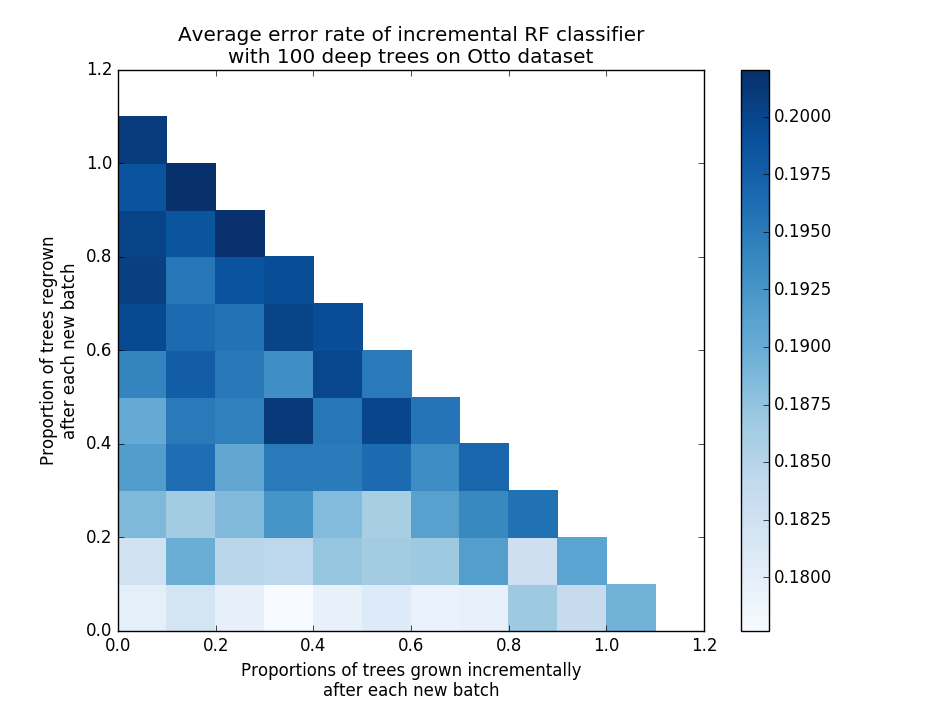
\includegraphics[width=5.0in]{otto_deep_med}\\
  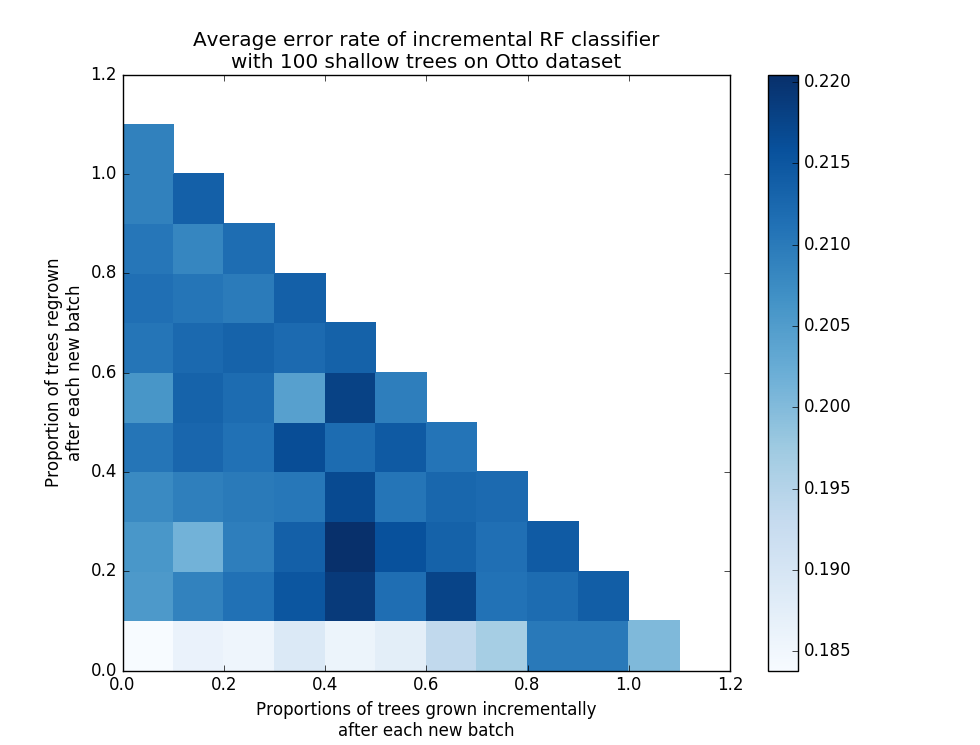
\includegraphics[width=5.0in]{otto_shallow_med}
  \caption{These two plots show the average error rates of various hybrid tree
  replacement and incremental growth strategies on the Otto Group batched
dataset. The axes indicate the percentage of trees that are modified according
to each strategy.}
  \label{fig:ottohybrid}
\end{figure}

Because the results do not indicate a clear dominant strategy, I instead
examine various hybrid approaches---strategies that combine both incrementally
growing and replacing trees.  As seen from the data in Figure
\ref{fig:ottohybrid}, for smaller batch sizes such as 100, strategies that
involve only incremental growth generally perform better than strategies that
incorporate some proportion of regrown trees. This trend is present in both
random forest classifiers comprised of deep trees and those with shallow trees,
though the trend is stronger among forests with shallow trees. 

Trees grown on one batch naturally overfit to that batch. With a small batch
size, there is a higher likelihood that data distribution differs from the
overall data distribution of the full dataset. As such, tree replacement
strategies could grow trees that fit well to one batch, but that fit poorly to
the rest of the data, increasing the error rate. Incremental growth
incorporates the data from multiple batches into each tree, mitigating the
effect of overfitting to the wrong data distribution.

Overall, these results demonstrate that data scientists using incremental
random forests on workloads with small data batches should utilize a strategy
that only involves incremental growth. Figure \ref{fig:ottohybrid} indicates
that the specific proportion of trees that are incrementally grown can vary
with little impact on accuracy, so data scientists should choose a smaller
ratio to minimize training time.

\section{Workload C: Large batches, concept drift}

The US Department of Transportation Airline On-Time Statistics and Delay Causes
dataset contains information about every flight that took place in the last
decade. I used 18-months of this dataset, beginning in January 2014, for my
analysis. Because the distribution of airline delay data varies seasonally,
this dataset exhibits concept drift. Each month of data translated to a
10,000-point batch in an 18-batch data workload. \cite{Plane}

\begin{figure}
  \centering
  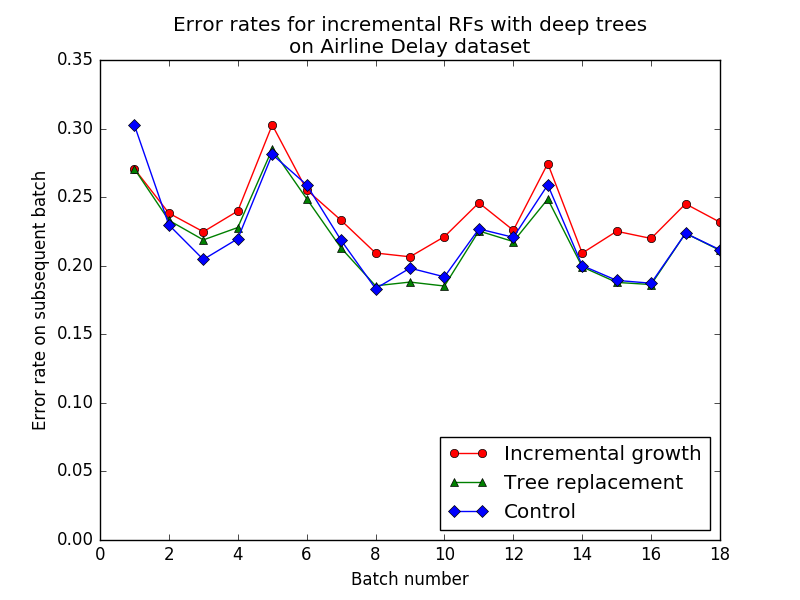
\includegraphics[width=4in]{planedeep_line}
  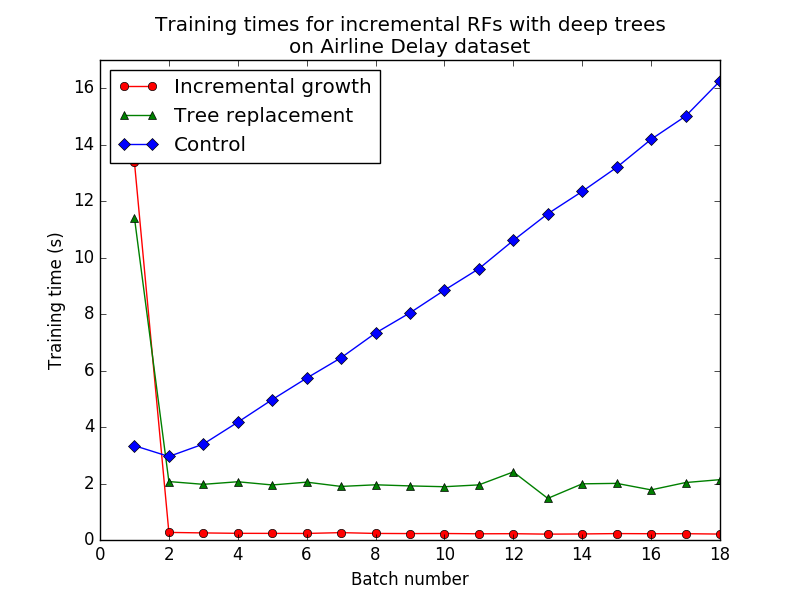
\includegraphics[width=4in]{planedeep_line_time}
  \caption{airline data}
  \caption{These graphs show the error rates and training times for the
incremental growth strategy, the tree replacement strategy, and the control
setting on the batched Airline Delay dataset. These metrics
were taken on online random forest classifiers growing deep trees.}
  \label{fig:plane1}
\end{figure}

\begin{figure}
  \centering
  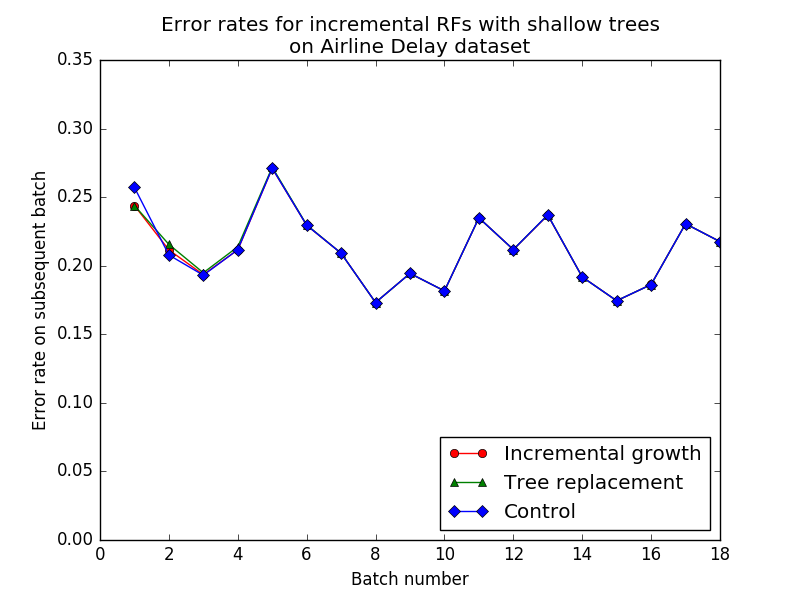
\includegraphics[width=4in]{planeshallow_line}
  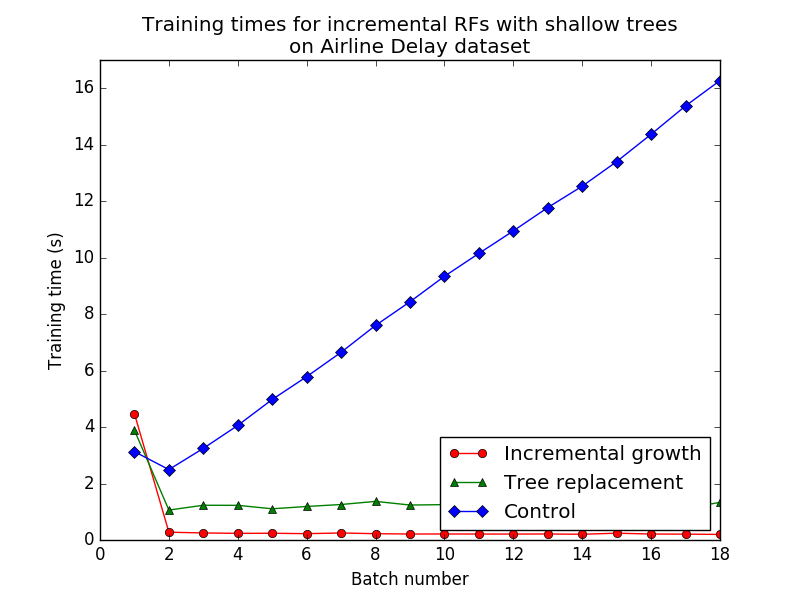
\includegraphics[width=4in]{planeshallow_line_time}
  \caption{airline data}
  \caption{As in the previous figure, these graphs show the error rates and
    training times for the two experimental strategies and the control on the
    batched Airline Delay dataset. These benchmarks were measured on online random forest
  classifiers growing shallow trees.}
  \label{fig:plane2}
\end{figure}


TODO plane data analysis


\begin{figure}
  \centering
  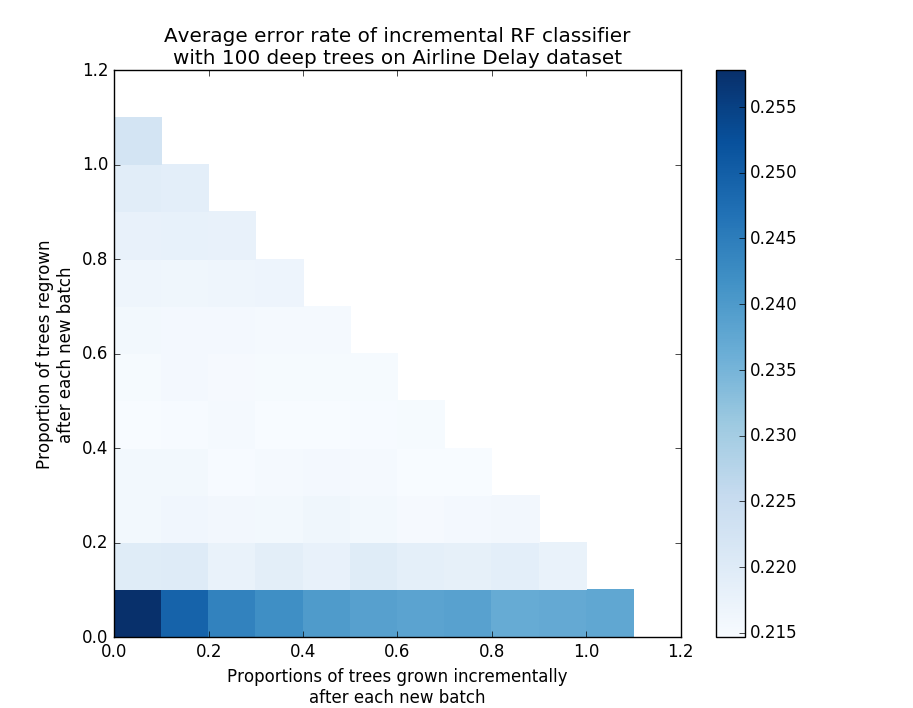
\includegraphics[width=5in]{planedeep}
  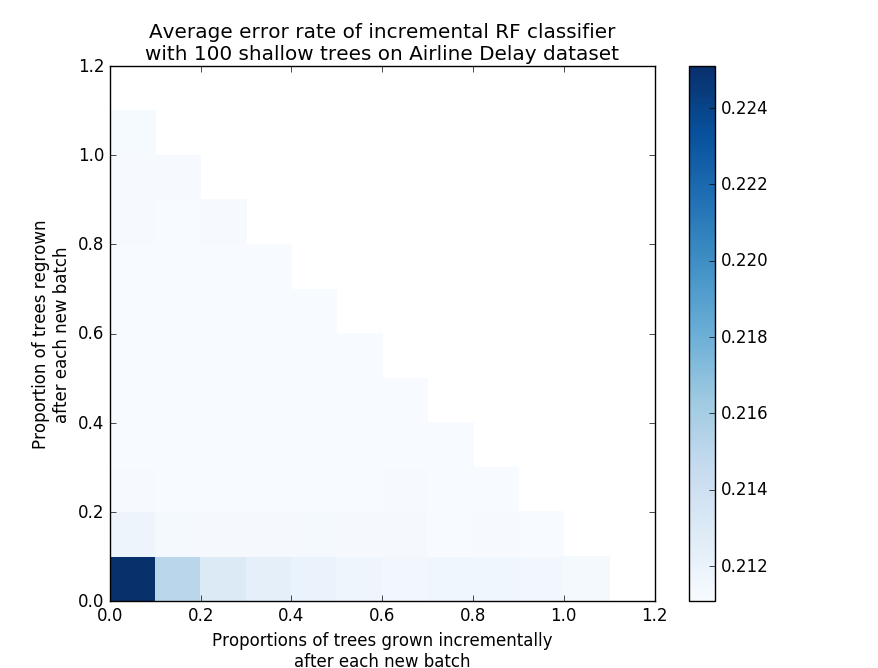
\includegraphics[width=5in]{planeshallow}
  \caption{These two plots show the average error rates of various hybrid tree
  replacement and incremental growth strategies on the Airline Delay batched
dataset. The axes indicate the percentage of trees that are modified according
to each strategy.}
  \label{fig:planehybrid}
\end{figure}
 
TODO force extreme concept drift with otto dataset



\section{Workload D: Small batches, concept drift}


TODO plane data analysis


\begin{figure}
  \centering
  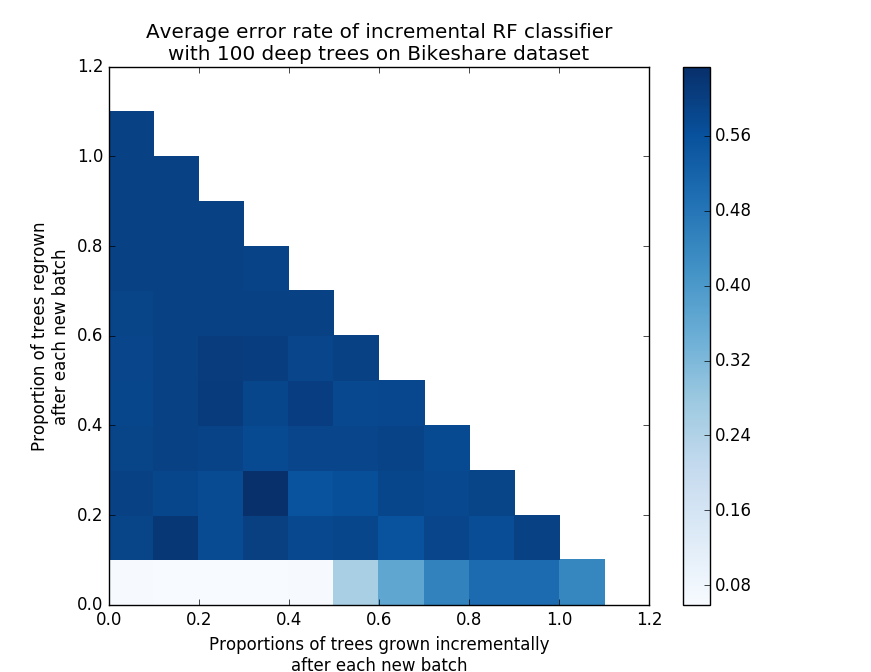
\includegraphics[width=5in]{bikesharedeep}
  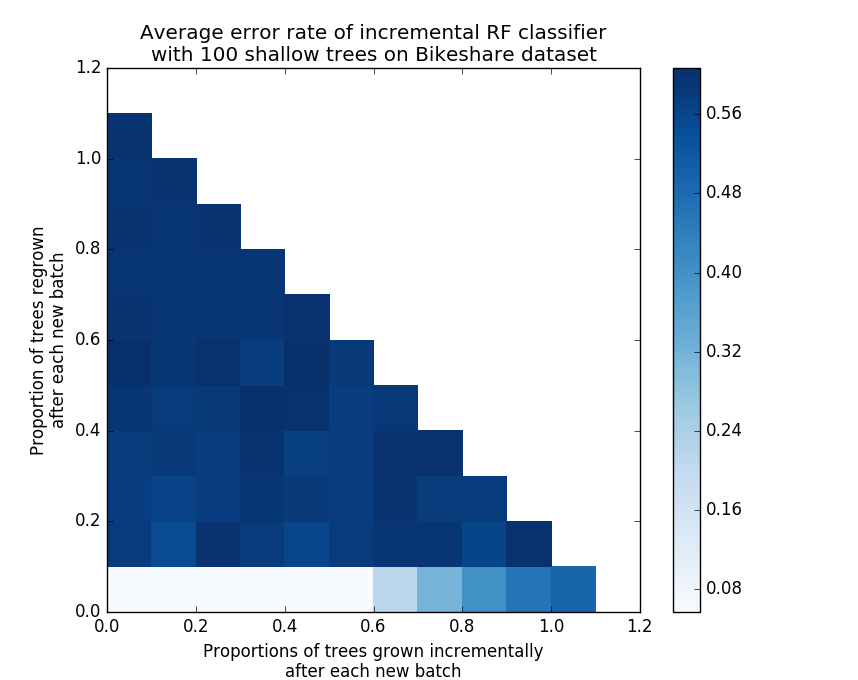
\includegraphics[width=5in]{bikeshareshallow}
  \caption{These two plots show the average error rates of various hybrid tree
  replacement and incremental growth strategies on the Bike Sharing batched
dataset. The axes indicate the percentage of trees that are modified according
to each strategy.}
  \label{fig:bikesharehybrid}
\end{figure}
 


\chapter{Conclusion}

\appendix
%% This defines the bibliography file (main.bib) and the bibliography style.
%% If you want to create a bibliography file by hand, change the contents of
%% this file to a `thebibliography' environment.  For more information 
%% see section 4.3 of the LaTeX manual.
\begin{singlespace}
\bibliography{main}
\bibliographystyle{plain}
\end{singlespace}

\end{document}

